% Options for packages loaded elsewhere
\PassOptionsToPackage{unicode}{hyperref}
\PassOptionsToPackage{hyphens}{url}
%
\documentclass[
]{article}
\usepackage{amsmath,amssymb}
\usepackage{iftex}
\ifPDFTeX
  \usepackage[T1]{fontenc}
  \usepackage[utf8]{inputenc}
  \usepackage{textcomp} % provide euro and other symbols
\else % if luatex or xetex
  \usepackage{unicode-math} % this also loads fontspec
  \defaultfontfeatures{Scale=MatchLowercase}
  \defaultfontfeatures[\rmfamily]{Ligatures=TeX,Scale=1}
\fi
\usepackage{lmodern}
\ifPDFTeX\else
  % xetex/luatex font selection
\fi
% Use upquote if available, for straight quotes in verbatim environments
\IfFileExists{upquote.sty}{\usepackage{upquote}}{}
\IfFileExists{microtype.sty}{% use microtype if available
  \usepackage[]{microtype}
  \UseMicrotypeSet[protrusion]{basicmath} % disable protrusion for tt fonts
}{}
\makeatletter
\@ifundefined{KOMAClassName}{% if non-KOMA class
  \IfFileExists{parskip.sty}{%
    \usepackage{parskip}
  }{% else
    \setlength{\parindent}{0pt}
    \setlength{\parskip}{6pt plus 2pt minus 1pt}}
}{% if KOMA class
  \KOMAoptions{parskip=half}}
\makeatother
\usepackage{xcolor}
\usepackage[left=30mm,right=30mm]{geometry}
\usepackage{graphicx}
\usepackage{float}
\setlength{\footskip}{50pt}
\makeatletter
\def\maxwidth{\ifdim\Gin@nat@width>\linewidth\linewidth\else\Gin@nat@width\fi}
\def\maxheight{\ifdim\Gin@nat@height>\textheight\textheight\else\Gin@nat@height\fi}
\makeatother
% Scale images if necessary, so that they will not overflow the page
% margins by default, and it is still possible to overwrite the defaults
% using explicit options in \includegraphics[width, height, ...]{}
\setkeys{Gin}{width=\maxwidth,height=\maxheight,keepaspectratio}
% Set default figure placement to htbp
\makeatletter
\def\fps@figure{htbp}
\makeatother
\setlength{\emergencystretch}{3em} % prevent overfull lines
\providecommand{\tightlist}{%
  \setlength{\itemsep}{0pt}\setlength{\parskip}{0pt}}
\setcounter{secnumdepth}{-\maxdimen} % remove section numbering
\ifLuaTeX
  \usepackage{selnolig}  % disable illegal ligatures
\fi
\IfFileExists{bookmark.sty}{\usepackage{bookmark}}{\usepackage{hyperref}}
\IfFileExists{xurl.sty}{\usepackage{xurl}}{} % add URL line breaks if available
\urlstyle{same}
\hypersetup{
  pdftitle={Reflective Report},
  hidelinks,
  pdfcreator={LaTeX via pandoc}}

\title{Realtime Rendering Reflective Report - Jacob Costen (23025180)}
\author{}
\date{}

\begin{document}
\maketitle

\hypertarget{realtime-rendering-reflective-report---jacob-costen-23025180}{%

\hypertarget{introduction}{%
\subsection{Introduction}\label{introduction}}

The practical artefact implements many basic features of rendering with
DirectX 11 (drawing geometry, using shaders to light pixels, altering
pipeline states, mapping textures) as well as several more advanced
techniques (SSAO, post-processing, normal mapping, shadow mapping, PBR
shader) and scene control functionality (object hierarchy, resource
management, JSON deserialisation). These features are demonstrated via a
scene created using Blender.

\hypertarget{uml}{%
\subsection{UML}\label{uml}}

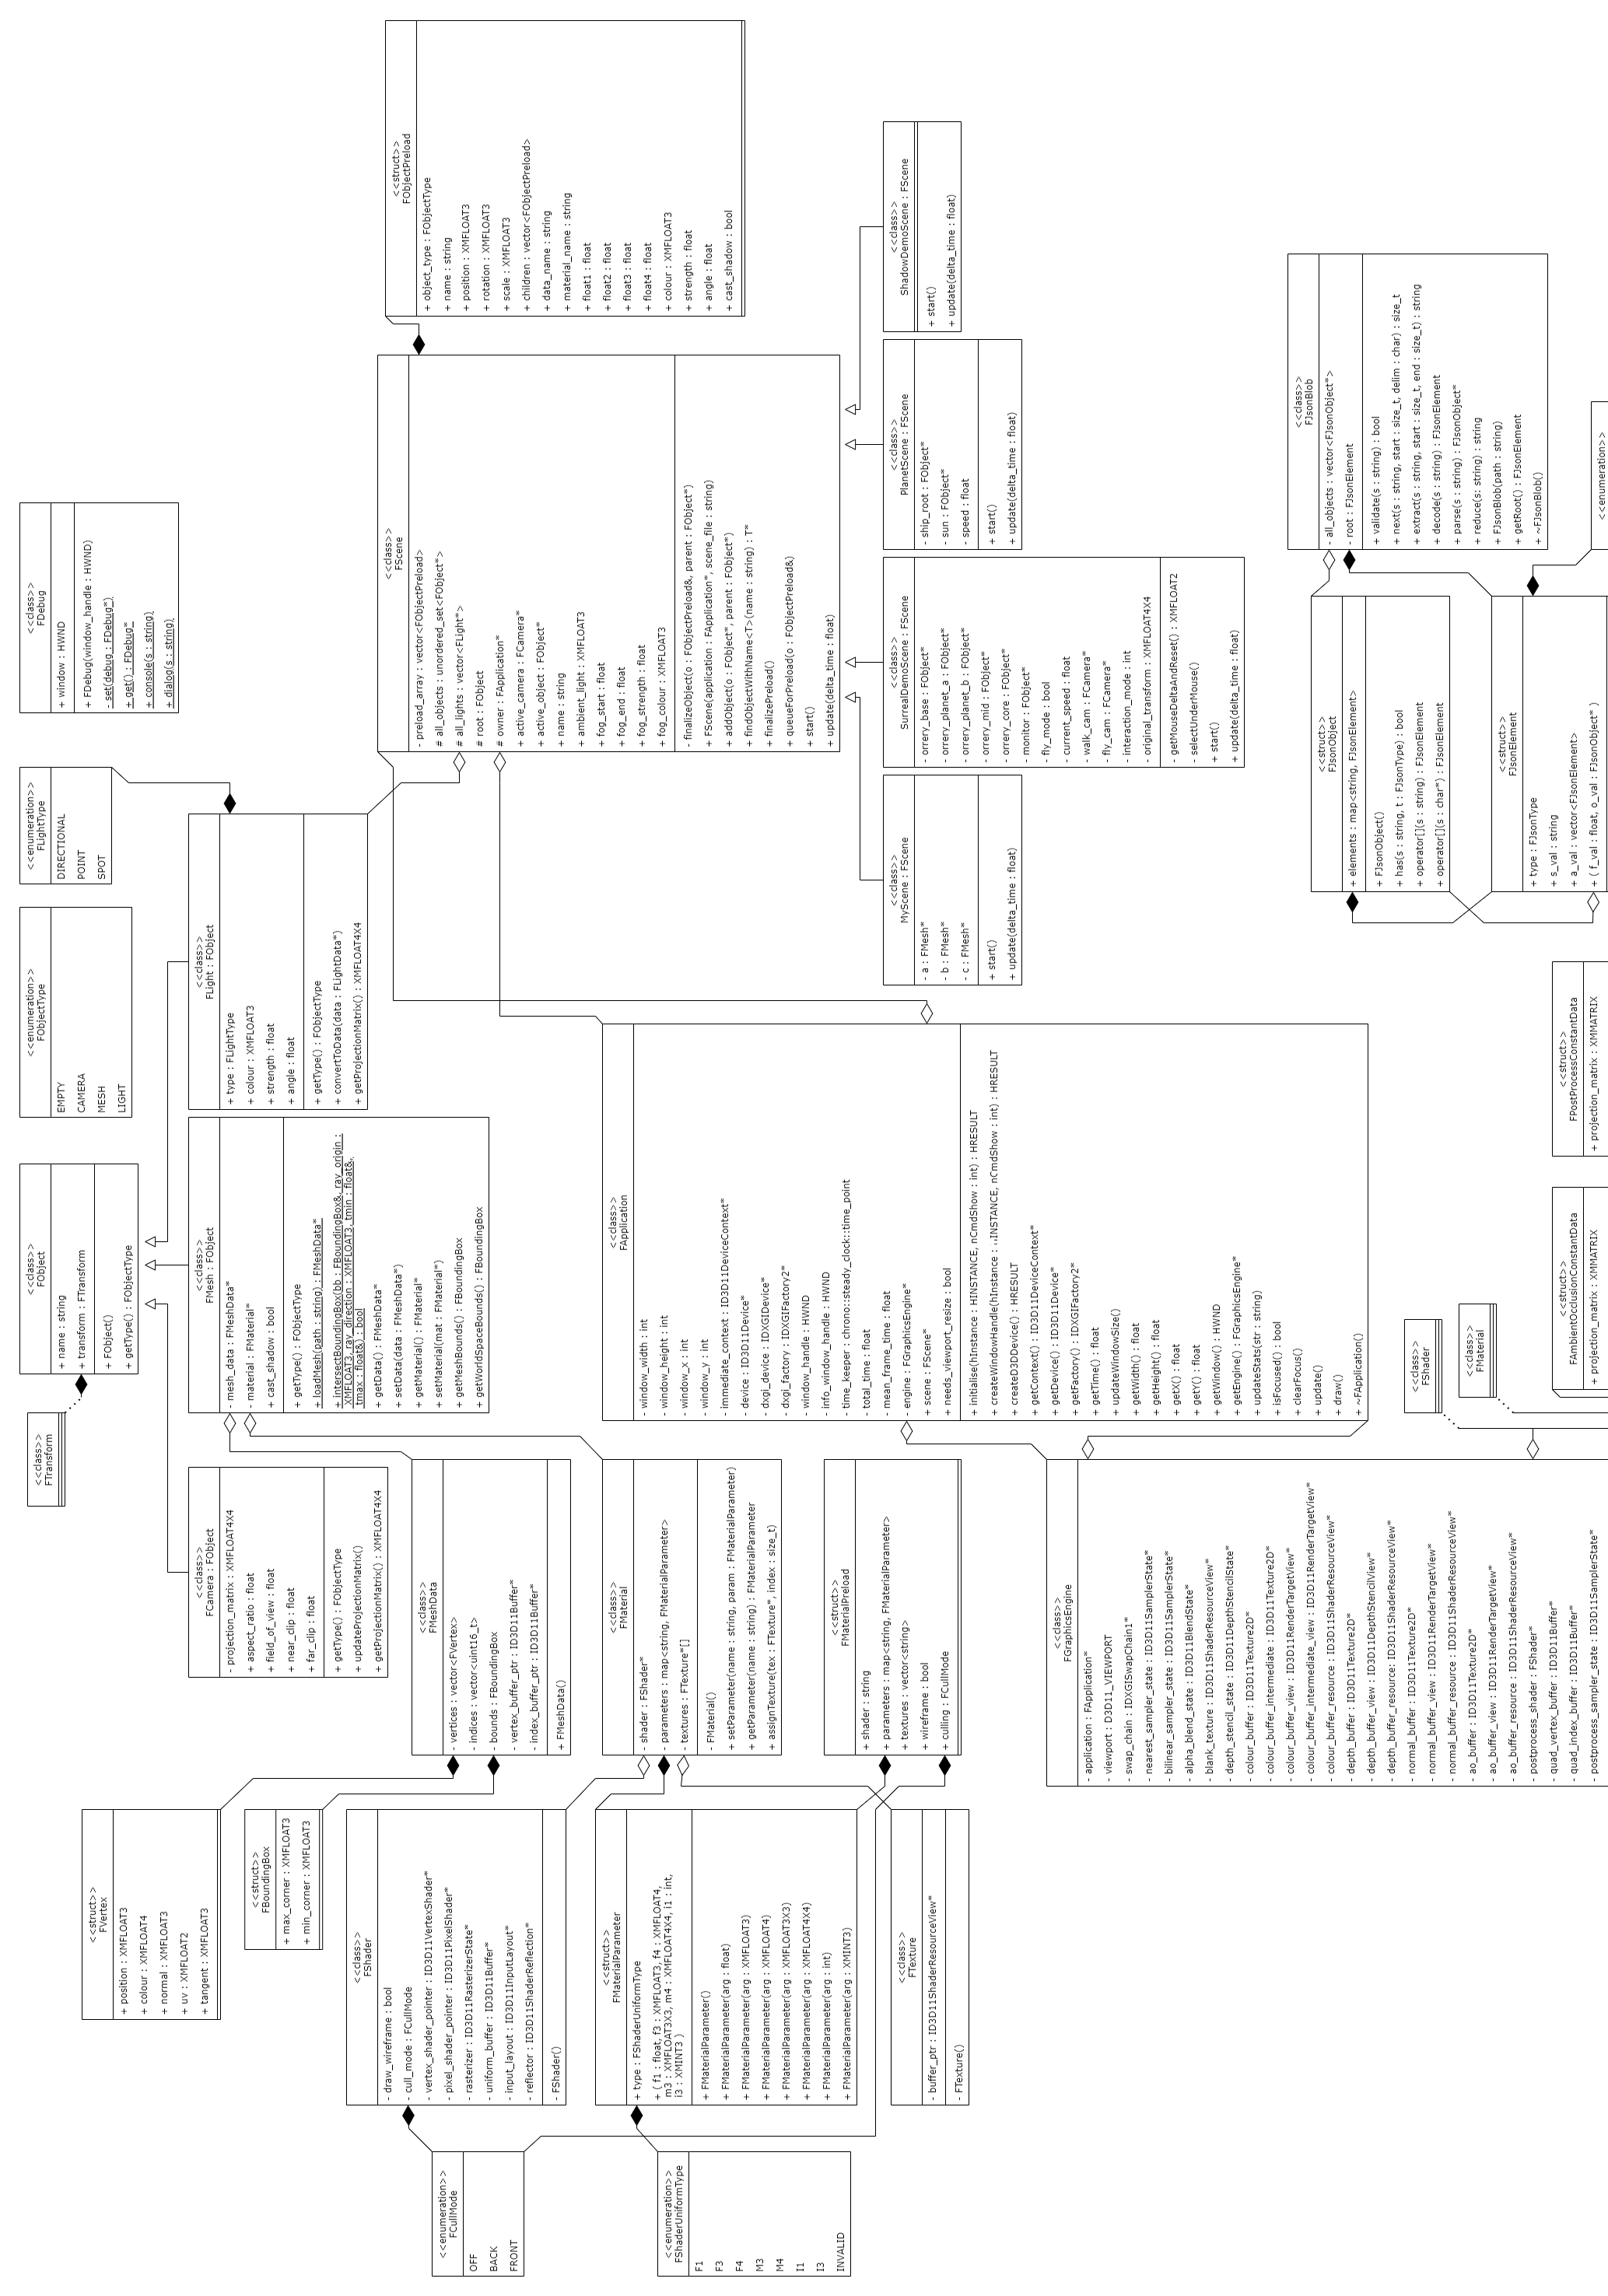
\includegraphics{/mnt/REPOSITORY/Repository-of-Things/Coding/C/gdev50038-artefact-oculometric/UML_a.png}\\
\newline
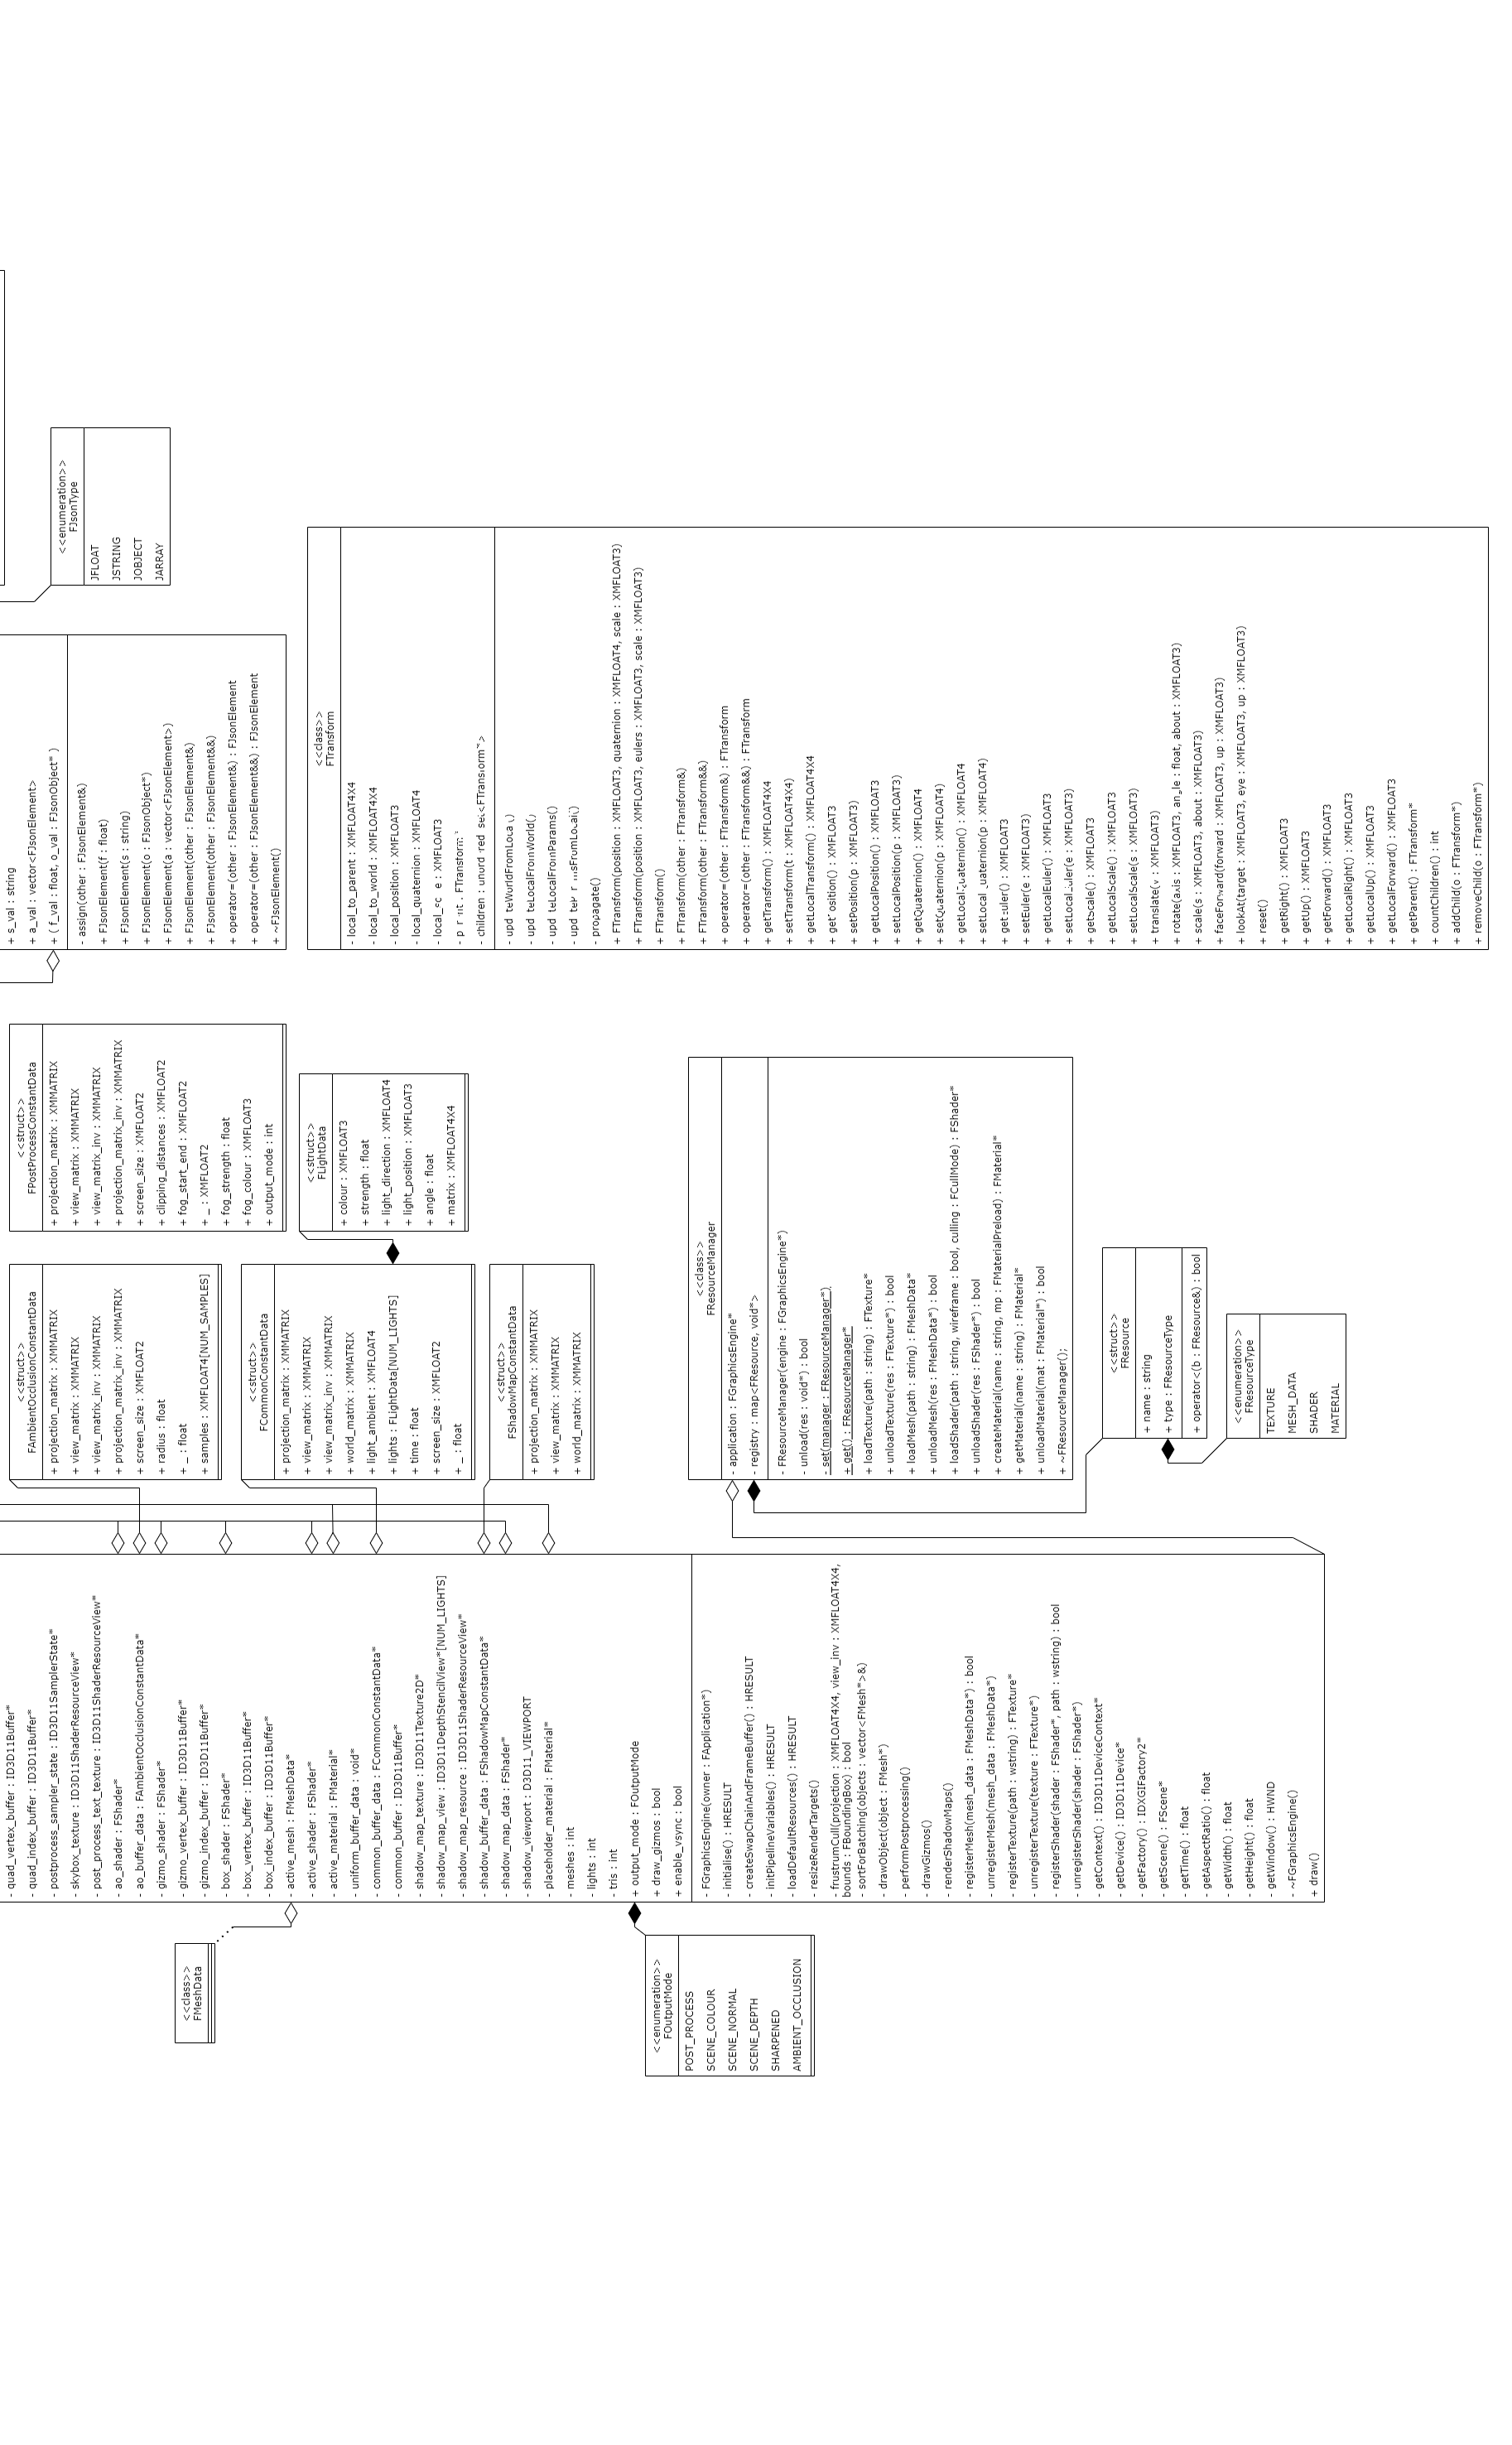
\includegraphics{/mnt/REPOSITORY/Repository-of-Things/Coding/C/gdev50038-artefact-oculometric/UML_b.png}\\
The artefact supports point, spot, and directional lights (up to 8
simultaneously, though this can be increased trivially) and shadow maps for spot/directional lights. Meshes are
shaded with a physically-based shader including albedo, normal mapping, roughness and metallic inputs, and the artefact makes use of both solid and wireframe rasterisers and both triangle and line assembler modes. The artefact makes use of the full-screen-quad technique to implement post-processing, and supports multiple render passes (colour, normal, depth, SSAO). The artefact also allows for resizing of the window/viewport, updating the various screen buffers accordingly. During drawing, scene objects are
sorted according to the shader used, to minimise the required context
switches. When debug view is enabled, object axes and bounding boxes are
drawn. These features are implemented via the \texttt{FGraphicsEngine}
class.

The post-processing shader includes a sharpening filter, and a
sophisticated ASCII-art shader inspired by a YouTube video by Acerola
(Gunnell (2024))\textsuperscript{{[}1{]}} which reduces the colour palette and uses ASCII characters as a matrix for dithering between neighbouring colours. It also features an
implementation of depth-based fog and a skybox. SSAO is performed in a
separate pass by a dedicated shader.

Most meshes make use of the \texttt{PhysicalShader.hlsl} shader, which
provides a thorough implementation of physically based rendering
according to the mathematical formulae described by de Vries
(2016)\textsuperscript{{[}2{]}}.

The engine is built around a scene graph, where a collection of
objects (empty, mesh, light, camera are all supported) are organised
hierarchically using per-object transforms, similar to the
\texttt{Transform} class provided by Unity (Unity
(2024))\textsuperscript{{[}3{]}}. Transforms have parents and children,
and may be transformed (translation, rotation, scaling) in both local
and world space, implemented by functions inside the \texttt{FTransform} class. This class also stores the world and local transform matrices of the object eliminating the need for these to be recalculated for rendering or transformation. The
\texttt{FScene} class manages objects, and provides functionality (start
and update) which can be overridden by subclasses to create custom
scenes (see \texttt{SurrealDemoScene}, \texttt{MyScene}, etc). It also provides functionality to create a list of objects to be created when the scene initialises, which is necessary for JSON loading.

Scenes may be stored on disk as JSON, which is deserialized at runtime.
Required assets are loaded as needed. Materials may also be configured
via JSON, allowing assignment of shader uniforms and textures. These
parameters are stored within an \texttt{FMaterial} instance. JSON files
are parsed by a custom algorithm, which includes support for block and
line comments.

Loaded assets (meshes, textures, shaders) are managed by the
\texttt{FResourceManager} class, preventing duplication and handling
unloading assets when the program finishes. The artefact features a
custom OBJ file loader, with the ability to load texture coordinates and
compute tangents at runtime, implemented by the \texttt{FMesh} and
\texttt{FMeshData} classes.

\hypertarget{successes}{%
\subsection{Successes}\label{successes}}

One feature which was implemented successfully was post-processing
support. This followed a standard technique where the scene is rendered
to an intermediate buffer (rather than one of the framebuffers) which is
then bound as a shader resource to be drawn on a single quad which fills
the screen, allowing use of the shading language, along with data
sampled from the intermediate buffers to produce a variety of stylistic
effects (Magdics, et al. (2013))\textsuperscript{{[}4{]}}. The artefact
closely follows this implementation, including the use of multiple
render passes: colour, normal, depth, and SSAO buffers are exposed to
the post-processing shader. The post-processing shader showcases an
interesting stylised ASCII-art effect, as well as a sharpen filter. The former uses ASCII letters as a dithering mask to blend between colours in a reduced colour palette. This shader
is where the fog and skybox are drawn, based on the values in the depth
buffer, eliminating the need for per-object fog or a separate skybox
object. However, the current post-processing shader does not demonstrate
use of the normal buffer for an effect, which is something that could be
improved. Additionally, an optimisation could be made such that instead
of the two triangles for a quad, a single triangle may be drawn which
overfills the screen. This would improve the performance of the
post-processing shader, but timing statistics show that the current
shader has an extremely trivial performance cost (compared with drawing
mesh objects).\\
\begin{figure}[H]
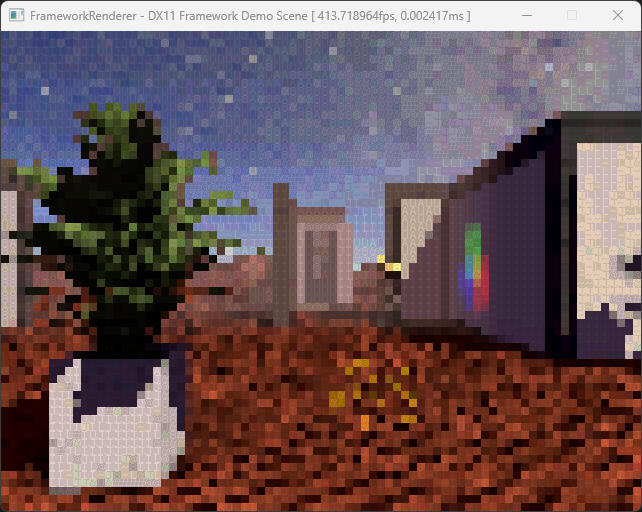
\includegraphics{/mnt/REPOSITORY/Repository-of-Things/Coding/C/gdev50038-artefact-oculometric/ascii_postprocess.png}
\caption{\label{fig:figure1} ASCII post-processing shader demo.}
\end{figure}

Another feature the artefact showcases is normal mapping. This is a
somewhat advanced technique which makes use of an additional texture (a
normal map) during shading to add the impression of denser surface
detail, without additional geometry. This is done by using tangents and
bitangents (vectors perpendicular to one another and to the surface
normal), which represent the direction of the U and V texture coordinate
axes in 3D space, to perturb the original surface normal according to
the normal map texture (de Vries (2013))\textsuperscript{{[}5{]}}. The
texture defines how to weight the sum of the normal, tangent, and
bitangent vectors to produce the new surface normal. The artefact
implements this using a T-B-N (tangent-bitangent-normal) matrix to
transform the normal map colour value (in tangent space) into a 3D
vector (in world space). This new normal is then used for lighting
calculations instead of the normal given by the vertex data.
Implementing this technique requires the provision of tangents, which
are calculated by the mesh reading code at load time in my custom OBJ model loader, according to the
algorithm described by Lengyel (2001)\textsuperscript{{[}6{]}}. This
technique provides excellent surface detail and improves realism,
however this additional calculation noticeably increases the time
required to load large meshes, and this is something which could be improved.

\begin{figure}[H]
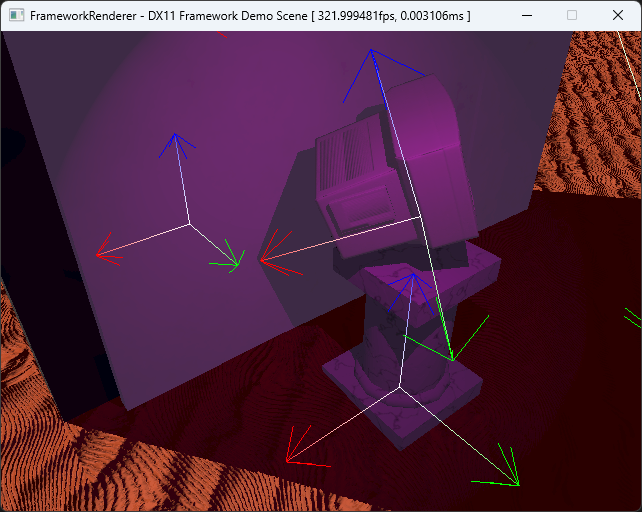
\includegraphics{/mnt/REPOSITORY/Repository-of-Things/Coding/C/gdev50038-artefact-oculometric/shadow_mapping.png}
\caption{\label{fig:figure2} Per-light shadow mapping.}
\end{figure}
The artefact also implements shadow mapping for spot and directional
lights. This technique takes advantage of the depth-buffering solution
to the visibility problem (the fundamental geometric problem which
rendering involves) to resolve shadows without expensive raytracing; the
scene is rendered from the perspective of each light, treating the light
as a camera, and the resulting depth buffer is stored in a texture. This
technique and its advantages are described by Everitt, Rege, and
Cebenoyan (2001)\textsuperscript{{[}7{]}}. Later, when individual
objects are rendered, this texture is sampled, and the value is compared
with the depth of the current geometry relative to the light. If the
depth of the geometry is greater than the value in the texture, then the
geometry must be shadowed. The artefact implements this technique by
rendering all objects with a simple dedicated shader, with only a depth
buffer bound. The artefact implements support for up to 8 lights total,
though this number can be increased arbitrarily. However, the current
implementation has limitations. The first of these is that spot lights
are not supported; implementing support for these would require
rendering the scene as a depth-cube-map from the light\textquotesingle s
position. The second limitation is that directional lights only render
shadows in a fixed area around themselves, meaning that they must be
positioned according to where the user wishes the shadow to have an
effect. Dimitrov (2007)\textsuperscript{{[}8{]}} presents a way to
resolve this by using multiple tiers of shadow maps (cascades) for
directional lights, and by adjusting the position of these cascades
according to the camera position to improve quality. Another limitation is that the artefact does not support blending/blurring to soften the jagged edges of shadows, a feature which most graphics engines offer which improves the visual look of mapped shadows and emulates the natural spread of lights which have non-zero source radius.\\

Another feature the artefact implements is screen space ambient
occlusion (SSAO). This effect involves sampling the depth and normal
buffers, generating randomly-offset samples in world space (relative to
the pixel normal), and then testing those sampled positions against the
depth buffer at that position. If the sample position is behind the
depth buffer, the sample is treated as occluded. The ambient occlusion
value is then provided by counting the number of samples which were not
occluded. This implementation is based loosely on that described by Luna
(2012)\textsuperscript{{[}9{]}}. An alteration made in the artefact is
the use of an ordered dithering matrix to compute random tangents/bitangents,
giving AO an even, dithered look. The ambient occlusion values are
output to a separate render target which is referenced by the
post-processing shader.\\
\begin{figure}[H]
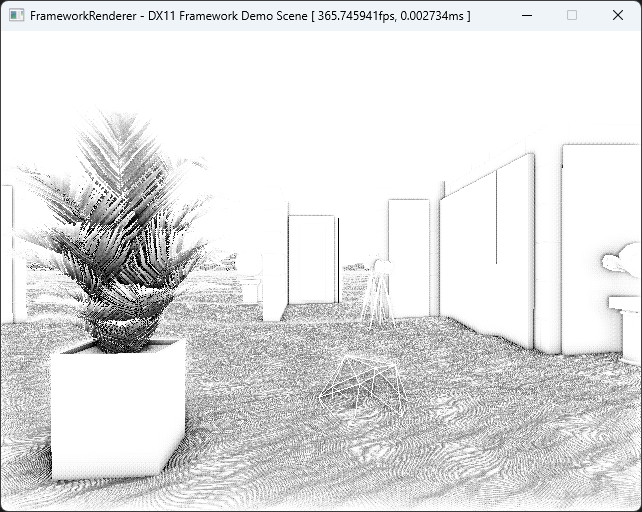
\includegraphics{/mnt/REPOSITORY/Repository-of-Things/Coding/C/gdev50038-artefact-oculometric/ambient_occlusion.png}
\caption{\label{fig:figure3} Screen-space ambient occlusion shader.}
\end{figure}

\hypertarget{limitations}{%
\subsection{Limitations}\label{limitations}}

One element of the framework which was never fully implemented was
frustrum culling. I tried to develop an algorithm which would test the
object\textquotesingle s axis-aligned bounding-box against the view
frustrum. Considering some test cases, I devised a solution where, after
the bounding box corners are transformed into clip space, they can be
trivially checked against the clip space bounds (if any AABB corners are
within the clip space cube, then the object must be drawn). However,
this solution missed several cases, for instance where the entire view
frustrum was contained within the AABB, or if the AABB was very narrow
and intersected across the middle of the frustrum without having
contained corners. Despite adding additional checks intended to catch
these edge cases, there still remain some scenarios where objects are
incorrectly culled, and the frustrum culling feature is disabled in the
current version of the project. In order to complete this
implementation, it would be ideal to find a source paper describing a
proven algorithm, such as the one presented by Sunar, Zin, and Sembok
(2008)\textsuperscript{{[}10{]}}.

\hypertarget{conclusion}{%
\subsection{Conclusion}\label{conclusion}}

The artefact successfully demonstrates a range of advanced techniques,
arguably the most significant of which is shadow mapping, since it helps
prevent the scene from looking flat, supplemented by the screen space
ambient occlusion. The sample scene, which was created from scratch
using Blender and inspired by surrealists like de Chirico, effectively
showcases the majority of the functionality presented in the artefact.
The sample scene skybox makes use of NASAs 2020 Deep Star Maps
(\url{https://svs.gsfc.nasa.gov/4851/} NASA/Goddard Space Flight Center
Scientific Visualization Studio. Gaia DR2: ESA/Gaia/DPAC. Constellation
figures based on those developed for the IAU by Alan MacRobert of Sky
and Telescope magazine (Roger Sinnott and Rick Fienberg)). All textures and models are my own work, aside from the teapot and monkey models, which are included with Blender.

\hypertarget{bibliography}{%
\subsection{Bibliography}\label{bibliography}}

{[}1{]}: Gunnell, G. (2024) \textquotesingle I Tried Turning Games Into
Text\textquotesingle, \emph{YouTube}. Available at:
\url{https://www.youtube.com/watch?v=gg40RWiaHRY} (Accessed: 11 November
2024).\\
{[}2{]}: de Vries, J. (n.d.). (2013) \emph{LearnOpenGL - Normal
Mapping}. learnopengl.com. Available at:
\url{https://learnopengl.com/Advanced-Lighting/Normal-Mapping}.\\
{[}3{]}: Technologies, Unity. (2024)
\textquotesingle Transform\textquotesingle, \emph{Unity Documentation}.
Available at:
\url{https://docs.unity3d.com/ScriptReference/Transform.html} (Accessed:
11 November 2024).\\
{[}4{]}: Magdics, M. \emph{et al.} (2013) `Post-processing NPR effects
for video games', \emph{Proceedings of the 12th ACM SIGGRAPH
International Conference on Virtual-Reality Continuum and Its
Applications in Industry}, pp. 147--156. doi:10.1145/2534329.2534348.\\
{[}5{]}: de Vries, J. (n.d.). (2016) \emph{LearnOpenGL - PBR Theory}.
learnopengl.com. Available at: \url{https://learnopengl.com/PBR/Theory}.\\
{[}6{]}: Lengyel, E. (2001) \emph{Mathematics for 3D game programming
and Computer Graphics, first edition}. Course Technology PTR.\\
{[}7{]}: Everitt, C., Rege, A., and Cebenoyan, C. (2001)
\textquotesingle Hardware shadow mapping\textquotesingle,~\emph{White
paper, nVIDIA},~\emph{2}.\\
{[}8{]}: Dimitrov, R. (2007) \textquotesingle Cascaded shadow
maps\textquotesingle,~\emph{Developer Documentation, NVIDIA Corp}.\\
{[}9{]}: Luna, F.D. (2012) \emph{Introduction to 3D game programming
with DirectX 11}. Dulles, Va: Mercury Learning and Information.\\
{[}10{]}: Sunar, M.S., Zin, A.M., and Sembok, T.M. (2008)
\textquotesingle Improved View Frustum Culling Technique for Real-Time
Virtual Heritage Application\textquotesingle,~\emph{Int. J. Virtual
Real.},~\emph{7}(3), pp.43-48.\\

\end{document}
